\documentclass[10pt]{beamer}

\usetheme{metropolis}
\usepackage{appendixnumberbeamer}

\usepackage{booktabs}
\usepackage{colortbl}
\usepackage{graphicx}
\usepackage{amsmath,mathtools}
\usepackage{tikz}
\usepackage{amsfonts}
\usepackage{cite}
\usepackage[scale=2]{ccicons}

\usetikzlibrary{shapes.geometric, arrows}
\tikzset{
  font={\fontsize{6pt}{12}\selectfont}}

\newcommand\scalemath[2]{\scalebox{#1}{\mbox{\ensuremath{\displaystyle #2}}}}

\usepackage{xspace}
\newcommand{\themename}{\textbf{\textsc{metropolis}}\xspace}

\title{A Robust Goal Programming Model For Transfer Pricing Risk Hedging:}
\subtitle{Preliminary Results}
\date{}
\author[shortname]{Marco Repetto \inst{1} \and  Davide La Torre \inst{2} \and  Danilo Liuzzi \inst{3}}
\institute[shortinst]{\inst{1} \textit{Department of Economics, Management and Statistics}, \textit{University of Milan-Bicocca}\\
Milan, Italy \\ m.repetto1@campus.unimib.it \and %

\inst{2} \textit{Dubai Business School, University of Dubai}\\
Dubai, UAE \\
dlatorre@ud.ac.ae \\
\textit{Department of Economics, Management, and Quantitative Methods, University of Milan}\\
Milan, Italy \\
davide.latorre@unimi.it \and %

\inst{3} \textit{Department of Economics and Management, University of Cagliari}\\
Cagliari, Italy \\
danilo.liuzzi@unica.it
}

% \titlegraphic{\hfill\includegraphics[height=1.5cm]{logo.pdf}}

\begin{document}

\maketitle

\begin{frame}{Table of contents}
  \setbeamertemplate{section in toc}[sections numbered]
  \tableofcontents[hideallsubsections]
\end{frame}

\section{Introduction}

\begin{frame}{Introduction}

  In the paper it is proposed a model for controlling the Transfer Pricing risk of a Multinational Firm operating in different countries and that has a well-defined value chain spread across its different controlled companies.

  These types of agreements controlling such transactions generally take into account different type of objectives. Because of the uncertainty embedded in these type of agreements a Robust Multicriteria Transfer Pricing risk model is built.
  
  The final result is a model in order to handle the possible worst-case scenarios in an environment of high uncertainty and mid to long-term planning.

\end{frame}

\section{Methods used}

\begin{frame}{Goal Programming}
\begin{columns}
\begin{column}{0.5\textwidth}
The Goal Programming \cite{charnes55} pertains to the field of Multicriteria Decision Analysis and is a distance-based method that relies on minimizing a set of deviation variables which model the distance between achieved levels and goals. The choice was to use the Weighted Goal Programming (WGP), because it allows for major trade-offs between each and every objective.
\end{column}
\begin{column}{0.5\textwidth}
\metroset{block=fill}
  \begin{alertblock}{WGP formulation}
  \begin{subequations}

\begin{align}
    & \underset{\delta}{\text{minimize}} & & w(\delta) \label{wgpmin} \\
    & \text{subject to} & & f_i(x)+ \delta_i=b_i, \; \forall i \in N \label{wgpsoftgoal} \\
    & & & x\in F \label{wgphardgoal}\\
    & & & \delta\geq 0 \label{wgppositivity}
\end{align}
\end{subequations}
\end{alertblock}
\end{column}
\end{columns}
\end{frame}

\begin{frame}{Robust Optimization}
\begin{columns}
\begin{column}{0.5\textwidth}
Robust Optimization builds on the philosophy of worst-case analysis. In contrast with Stochastic Programming \cite{dantzig55} which assumes probabilistic modelling of the uncertainty; RO poses that parameters vary arbitrarily in known bounded sets, called uncertainty sets \cite{soyster73}. RO gained momentum in recent years thanks to the extended work of Ben-Tan and Nemirovski \cite{ben-tal97}\cite{ben-tal98}\cite{ben-tal99}.
\end{column}
\begin{column}{0.5\textwidth}
\metroset{block=fill}
  \begin{alertblock}{Robust formulation of a linear programming model}
\begin{subequations}
\begin{align}
    & \underset{x}{\text{minimize}} & & f(x) \label{rpmin} \\
    & \text{subject to} & & g(x)=\chi(\xi), \; \xi \in \Xi \label{rpcon} \\
\end{align}
\end{subequations}
  \end{alertblock}
\end{column}
\end{columns}
\end{frame}

\begin{frame}{Robust Goal Programming}
  The RO problem shown above has two major drawbacks, namely:
  \begin{enumerate}
  \item It does not include any measure of robustness which the
    DM can act on;
  \item It does not allow (by design) to consider multiple objectives.
  \end{enumerate}
  A hybrid approach that tries to fix both of these problems affecting early stage Robust Optimization formulations was originally developed by Kuchta \cite{kuchta04}.
  In this formulation, the robust tuning parameter is played by \(r\) where \(r=0...n\) given \(n\) the number of parameters subjected to uncertainty.

\end{frame}
\begin{frame}[allowframebreaks]{Robust Goal Programming}
\metroset{block=fill}
  \begin{alertblock}{Compact formulation of a Robust Goal Programming model}
\begin{subequations}

\begin{align}
    & \underset{\delta}{\text{minimize}} & & w(\delta) \label{wrgpmin} \\
    & \text{subject to} & & f_i(x) + \sum_{j=1}^{Q}p_{ij} + r_iz_i + \delta_i = b_i, \forall i \in N  \label{wrgpsoftgoal} \\
    & & & z_i + p_{ij} \geq g_{ij}(x), \forall i \in N , \forall j \in Q \label{wrgptuning} \\
    & & & x\in F \label{wrgphardgoal} \\
    & & & \delta_i, p_{ij}, z_i \in \mathbb{R}^{+} \label{wrgppositivity} \\
    & & & x \in \mathbb{R}^{s} \label{wrgpfeasible}
\end{align}
\end{subequations}
  \end{alertblock}

  \pagebreak
  
  The deviations in Equation (\ref{wrgpmin}) are weighted using the function $w$. The tuning parameter that permits to adapt the price of robustness \cite{bertsimas04} is represented by \(r\), and Equation (\ref{wrgphardgoal}) models the presence of more abstract constraints. 
  
\end{frame}

\section{Transfer Pricing Policies}

\begin{frame}{Transfer Pricing Policies}
  Generally, Multinational Entities (MNE) subject to TP legislative burden tend to act proactively promoting agreements that bind the counterparts belonging to the same group for particular value-related process, in these agreements it is possible to identify different aspects:
  \begin{enumerate}
  \item The counterparts;
  \item The role of the counterparts;
  \item The remuneration of the counterparts;
  \item Auxiliary clauses.
  \end{enumerate}
The aspect of remuneration is crucial in these policies because may lead tax avoidance conducts. In the best practices provided by the OECD\cite{oecd17} several methods are proposed to cope with this aspect as presented in Figure \ref{fig:tp-m}.
\end{frame}

\begin{frame}[fragile]{Transfer Pricing Methods}
\begin{figure}
\centering
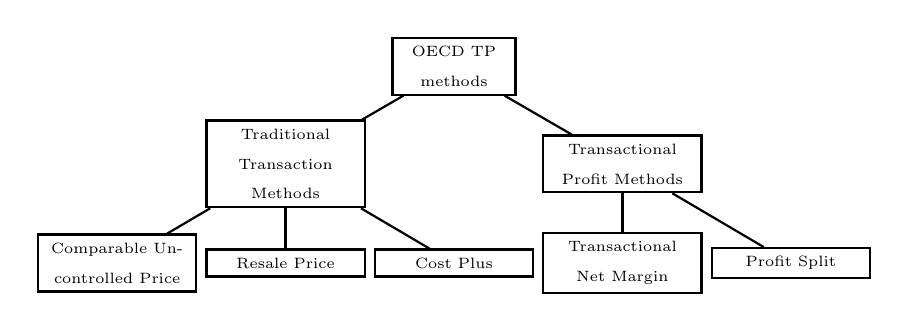
\begin{tikzpicture}[thick, every node/.style={scale=0.9}]
  \matrix [column sep=1mm, row sep=3mm] {
    & &
  \node (yw) [draw, shape=rectangle,text width=1.5cm,align=center] {OECD TP methods}; &
  & \\
  &
   \node (d1) [draw, shape=rectangle,text width=2cm,align=center] {Traditional Transaction Methods}; & &
  \node (d2) [draw, shape=rectangle,text width=2cm,align=center] {Transactional Profit Methods}; & \\
  \node (we) [draw, shape=rectangle,text width=2cm,align=center] {Comparable Uncontrolled Price}; &
  \node (wf) [draw, shape=rectangle,text width=2cm,align=center] {Resale Price}; &
  \node (wg) [draw, shape=rectangle,text width=2cm,align=center] {Cost Plus}; &
  \node (pu) [draw, shape=rectangle,text width=2cm,align=center] {Transactional Net Margin}; &
  \node (pl) [draw, shape=rectangle,text width=2cm,align=center] {Profit Split}; \\
};
\draw[-, thick] (d1) -- (we);
\draw[-, thick] (yw) -- (d1);
\draw[-, thick] (yw) -- (d2);
\draw[-, thick] (pu) -- (d2);
\draw[-, thick] (d1) -- (wg);
\draw[-, thick] (d1) -- (wf);
\draw[-, thick] (d2) -- (pl);
\end{tikzpicture}
\caption{TP methods in the OECD guidelines.} \label{fig:tp-m}
\end{figure}
\end{frame}

\begin{frame}{Transfer Pricing Methods}
  In the case under analysis we excluded the Traditional Transaction Methods because of a lack of comparable transactions involving the MNE and other third parties unrelated companies. Therefore the choice was to opt for Transactional Profit Methods.

  The Transactional Net Margin Method (TNMM) is based on the examination of the net profit relative to an appropriate base (e.g. costs, sales, assets) that a local entity realizes from a controlled transaction (or in our case to the entity itself).

  In order to achieve this is necessary to identify which Profit Level Indicator to choose; this is an important choice that has to be made taking into account the functional characterization of such entity. The main PLIs used by the practitioners are: Return on Sales (ROS), Full Cost Mark-up (FCMU), Return on Asset (ROA) and Return on Investment (ROI).
\end{frame}

\section{The Model}

\begin{frame}{The Model}
  When dealing with the setting of the transfer prices, the DM faces a series of choices that most of the times conflict with each other, ranging from management profitability requirements to greedy tax minimization, hence a GP model has been chosen.

  Apart from the number of objectives considered a key role is played by the dynamics of the environment in which such decisions are taken, such environment tends to be influenced by a certain degree of uncertainty, and therefore the TP policies have to be robust in the sense that has to account for that uncertainty.
\end{frame}

\begin{frame}[allowframebreaks]{Deterministic Formulation}
  \begin{subequations}
    The deterministic WGP model formulation reads as:
    
\scalebox{0.7}{\parbox{1\linewidth}{%
\begin{align}
    & \underset{\delta^+,\delta^-}{\text{minimize}} & & \sum^{N}_{i=1}w_i(\delta^+_i + \delta^-_i) & \label{dm_obj} \\
    & \text{subject to} & & n\cdot \sum^{Q}_{j=1}(x_j\cdot t_j) - \prescript{t}{}{\delta^+}  =\overset{\star}{t} & \label{dm_tax} \\
    & & & n\cdot \frac{x_j}{b_j} - \prescript{m}{}{\delta^+_j} + \prescript{m}{}{\delta^-_j} = m_j, & \forall j \in Q \label{dm_median} \\
    & & & {x_j} - \prescript{g}{}{\delta^+_j} + \prescript{g}{}{\delta^-_j} = g_j, & \forall j \in Q \label{dm_management} \\
    & & & \sum^{Q}_{j=1} c_j(x_j) \geq p & \label{p_l} \\ 
    & & & \sum^{Q}_{j=1} c_j(x_j) \leq p + \Delta & \label{p_u} \\
    & & & n\cdot \frac{x_j}{b_j} \geq l_j, & \forall j \in Q \label{l_q} \\
    & & & n\cdot \frac{x_j}{b_j} \leq u_j, & \forall j \in Q \label{up_q}\\
    & & & \delta^+_i,\delta^-_i,x_j\geq 0  & \forall i \in N, \quad \forall j \in Q
\end{align}
}}
\end{subequations}

\pagebreak

The three types of deviational variables (i.e. \(^t\),
\(^m\), \(^g\)) belong to main objectives which are:

\begin{itemize}
\item Tax minimization;
\item Transfer Pricing compliance;
\item Management goals.
\end{itemize}

Equation (\ref{dm_tax}) refers to the tax minimization and $\overset{\star}{t}$ has to be intended as the absolute value of tax expenses that MNE would like to pay whereas $x_j$ represent the margin allocated in absolute value to each function per unit of product.

The l.h.s. represent the current tax liability identified as:
  $$
  n\cdot \sum^{Q}_{j=1}(x_j\cdot t_j)  = \text{EBIT} \cdot \text{Tax Rate} = \text {Tax Liability} 
  $$
  Equation (\ref{dm_median}) refers to the TNMM goal for the net profit indicator to be in line with the median of a particular set of independent companies $m_j$, whereas the l.h.s. side represents the Earnings Before Interest and Taxes over the applicable base defined by TNMM which is:
  $$
  n\cdot \frac{x_j}{b_j} = \frac{\text{EBIT}_j}{\text{BASE}_j} \quad j \in Q \quad b = \begin{bmatrix} \text{Return On Sales} \\ \text{Return On Assets} \\ \vdots \end{bmatrix}
  $$
  Equations (\ref{l_q}) and (\ref{up_q}) represent the lower and upper quartile indicator boundary of the TNMM. Equation (\ref{dm_management}) sets the management's objectives for each off-shore division in terms of margin per product. Equation (\ref{p_l}) and (\ref{p_u}) sets minimum and maximum price deviation accepted because of the TP policy. The decision variables \(x\) represent the margin of the product allocated to the j-th firm.

\end{frame}

\begin{frame}{Robust Formulation}

\begin{columns}
\begin{column}{0.5\textwidth}
  The model presented above was robustified against three
  different factors:
  \begin{enumerate}
  \item Uncertainty related to tax rate;
  \item Uncertainty related to duties;
  \item Uncertainty regarding the feasible range of compliance with the TNMM.
  \end{enumerate}

  The resulting robust WGP model formulation is proposed on the right.
  
\end{column}
\begin{column}{0.5\textwidth}
\begin{subequations}

  \scalebox{0.6}{\parbox{1.8\linewidth}{%
\begin{align}
& \underset{\delta^+,\delta^-}{\text{minimize}} \sum^{N}_{i=1}w_i(\delta^+_i + \delta^-_i)\\
& \text{subject to} \sum^{Q}_{j=1}(x_j t_j + \pi_{1,j})+ \prescript{t}{}{\rho} \prescript{t}{}{\zeta} - \prescript{t}{}{\delta^+}  =\overset{\star}{t} \\
& n\cdot \frac{x_j}{b_j}+\pi_{2,j}+ \prescript{m}{}{\rho} \prescript{m}{}{\zeta} - \prescript{m}{}{\delta^+} + \prescript{m}{}{\delta^-_j} = {m_j}, & \forall j \in Q \\
& {x_j} - \prescript{g}{}{\delta^+_j} + \prescript{g}{}{\delta^-_j}  = {g_j}, & \forall j \in Q \\
& \sum^{Q}_{j=1} c_j(x_j) + \pi_{3,j} + \prescript{t}{}{\rho} \prescript{g}{}{\zeta} \geq p \\
& \sum^{Q}_{j=1} c_j(x_j) + \pi_{3,j} + \prescript{t}{}{\rho} \prescript{g}{}{\zeta} \leq p + \Delta \\
& n\cdot \frac{x_j}{b_j} \geq {l_{j,u}}, \qquad  \forall j \in Q, \quad \forall u \in U \label{lquartile} \\
& n\cdot \frac{x_j}{b_j} \leq {u_{j,u}}, \qquad \forall j \in Q, \quad \forall u \in U \label{uquartile} \\
& \zeta_i + \pi_{ij} \geq \theta_{ij} x_{j},  \qquad \forall i \in N, \quad \forall j \in Q \\
& \delta^+_i,\delta^-_i,x_j\geq 0, \qquad \forall i \in N, \quad \forall j \in Q
\end{align}
}}
\end{subequations}
\end{column}
\end{columns}
\end{frame}

\section{Model Deploy}

\begin{frame}{Model Deploy}
The deploy of the model was pursued through Julia\footnote{Version 1.0.3 (2018-12-18), built on GNU/Linux Fedora 29.}\cite{bezanson17}. The full stack used for the deployment of the model was divided as such:
\begin{itemize}
\item Algebraic modelling stack: the formalization of the robust model was obtained by using JuMP\cite{dunning17}\cite{lubin15}, a modeling language for mathematical optimization embedded into Julia and for the implementation of the Lexicographic approach the vOptSolver\cite{xavier17} library was used.
\item Solvers stack: the solver stack was primarily divided into two solvers:
  \begin{itemize}
  \item COIN-OR\cite{heimer2003} Linear Programming solver: the interface was provided by the Clp.jl package embedded into the JuliaOpt library;
  \item GNU Linear Programming Kit: the interface was provided by the Julia GLPK module embedded into the JuliaOpt library.
  \end{itemize}
\end{itemize}
\end{frame}

\section{Results}

\begin{frame}[allowframebreaks]{Weight sensitivity analysis}
  Since the approach applied was a weighted one, it was performed a sensitivity analysis \cite{jones11} in order to test the possible achievable objectives and their trade-offs with respect to the weights.

  In the ternary plot depicted at Figure \ref{tern} are presented the various combinations of weights and the sum of the decisional variables. Such sensitivity was tested by assuming no robustness of the model (\emph{i.e.} $\rho = [0,0,0]$).

  \pagebreak
  
\begin{columns}
\begin{column}{0.4\textwidth}   
There is a decrease in profit allocation in case of a greater tax liability concern. Conversely, other weighting schemes tend to not change the value of the objective function but just how the profits are allocated among the entities.
\end{column}
\begin{column}{0.6\textwidth}

  \begin{figure}
\centering
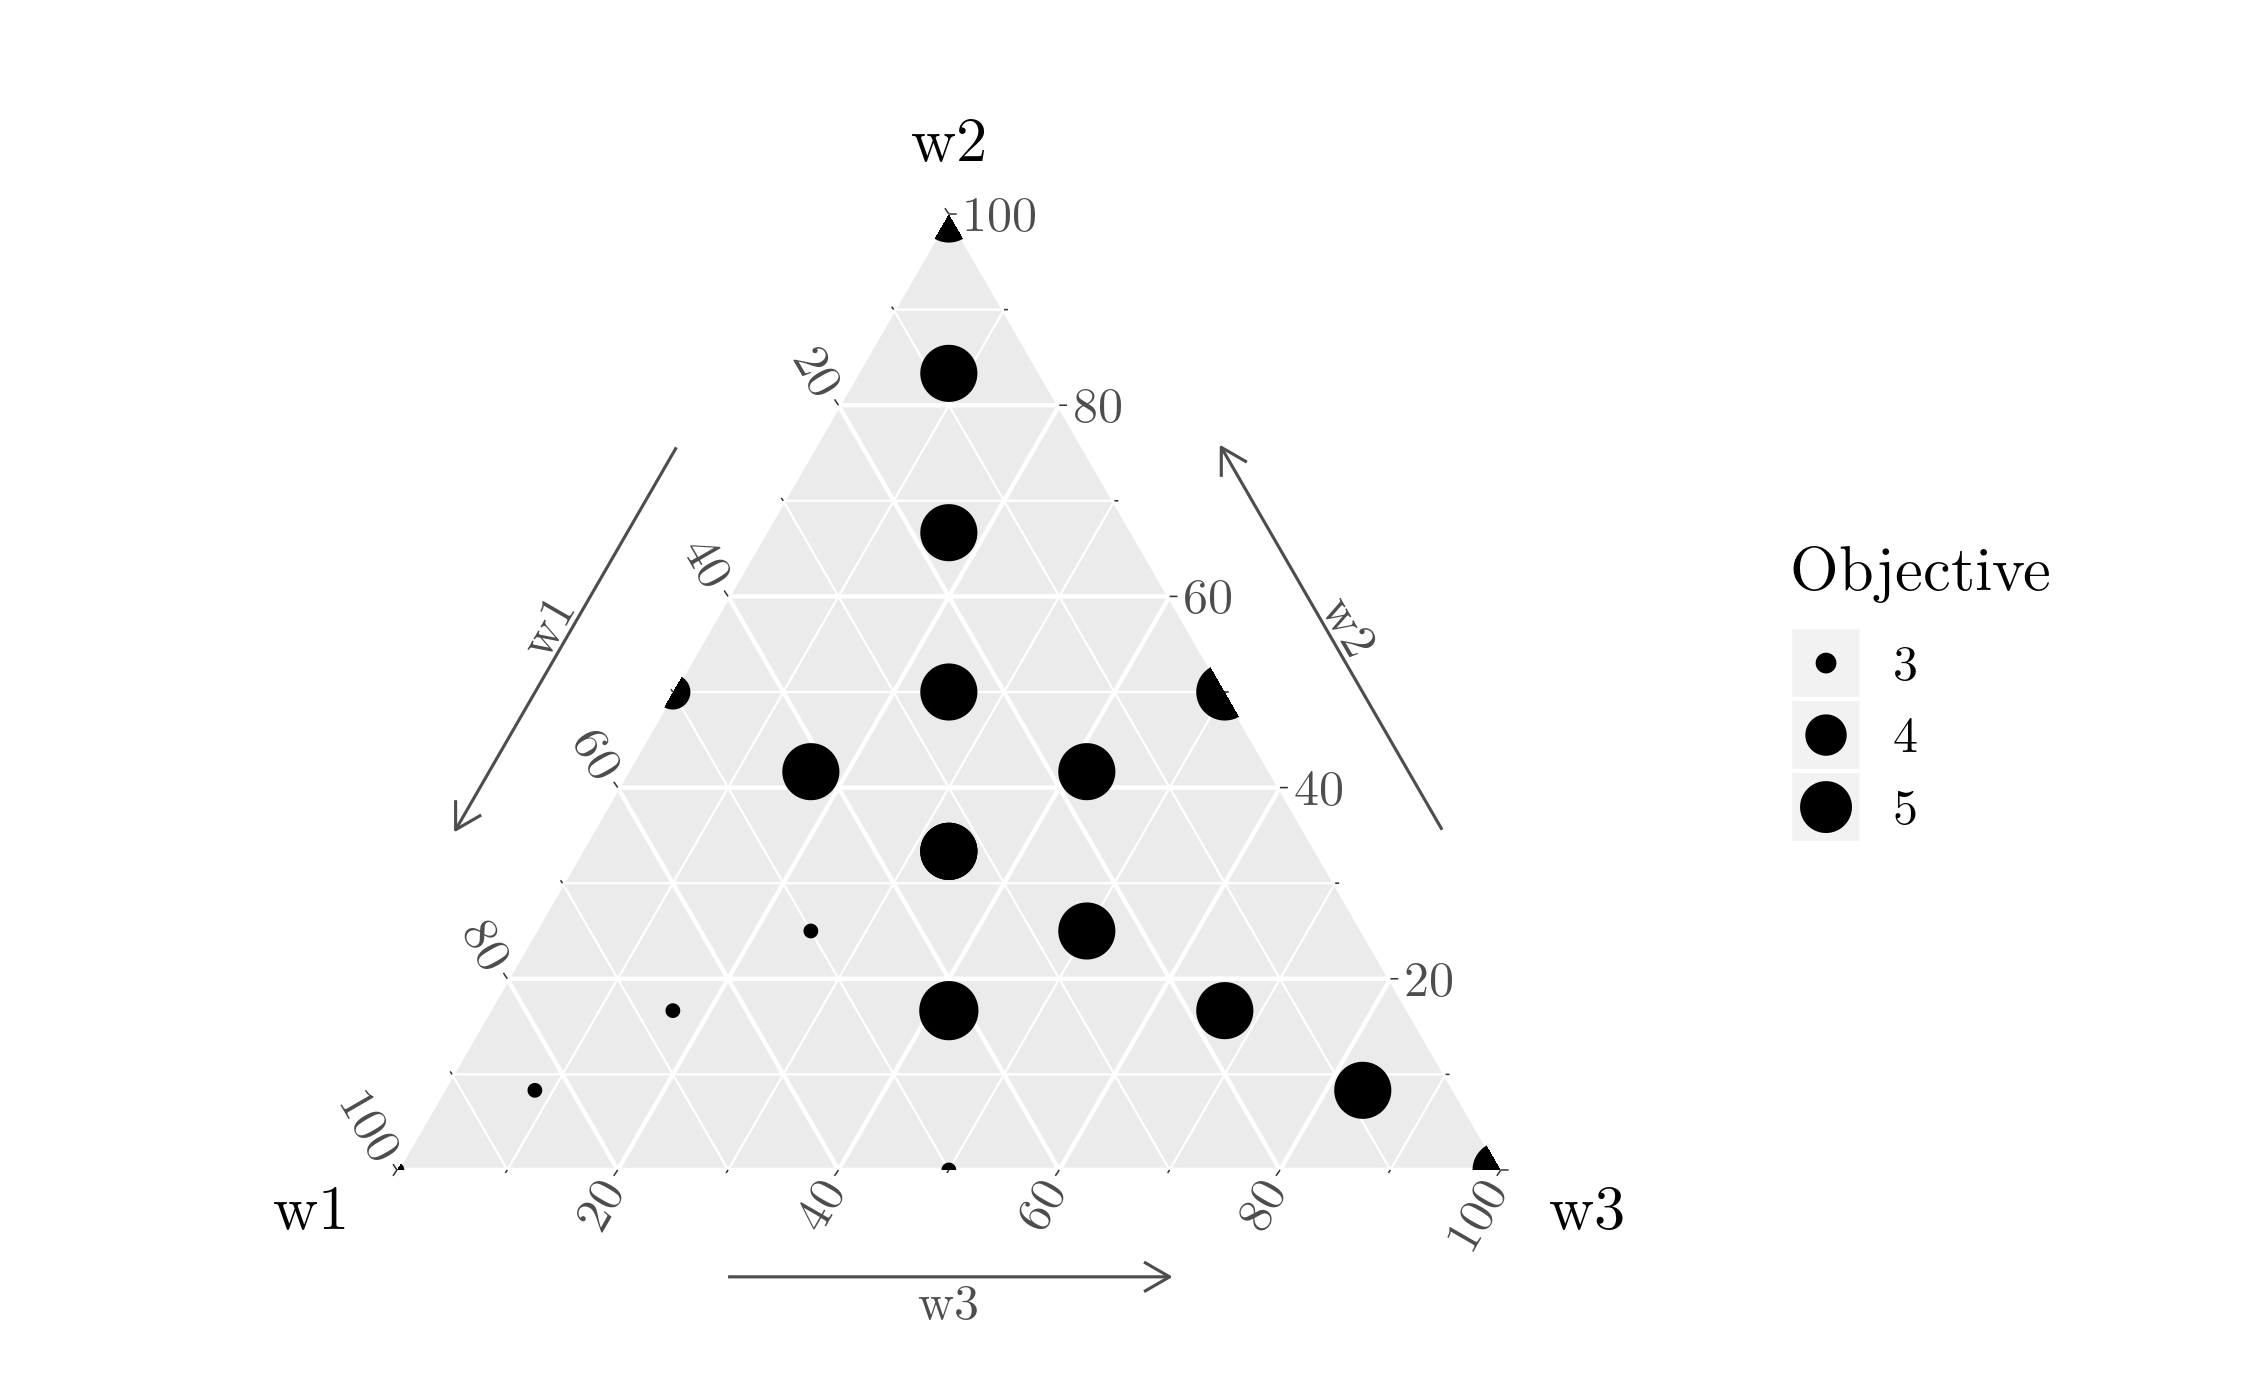
\includegraphics[width=2.5in]{figure/ternary.png}
\DeclareGraphicsExtensions.
\caption{Weight sensitivity ternary plot.}
\label{tern}
\end{figure}

\end{column}
\end{columns}
\end{frame}

\begin{frame}[allowframebreaks]{Final results}
  As emerged in the literature, the main goal of the agents setting the TP policy is not always a mere focus on achieving a lower tax burden but instead on be as compliant as possible with the best practices in order to avoid any tax-related risk.

  Therefore the choice was to give major importance to the second objective then leaving the other two, namely management goal and tax liability minimization, the same importance.

\begin{figure}[]
\centering
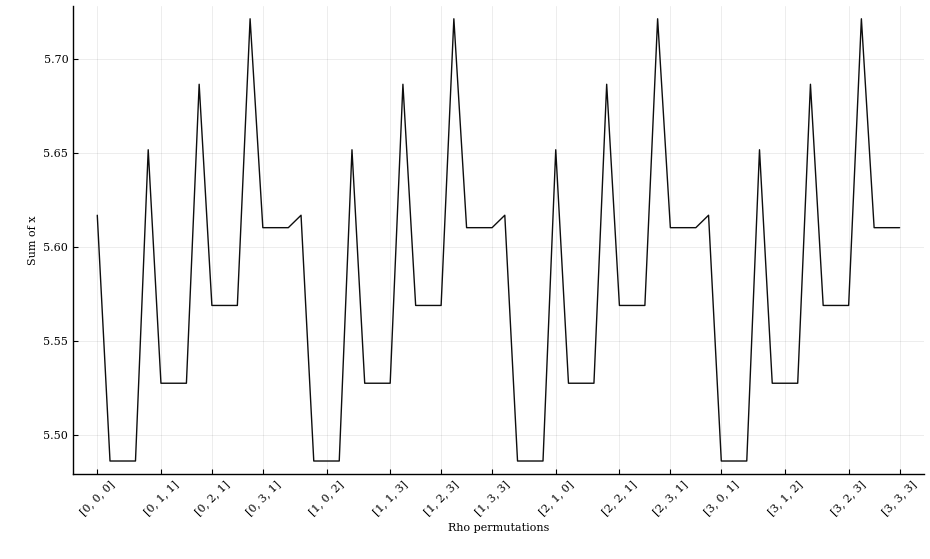
\includegraphics[width=3in]{figure/Figure_1.png}
\DeclareGraphicsExtensions.
\caption{Rho permutations and objective function results.}
\label{last}
\end{figure}
\end{frame}

\begin{frame}[allowframebreaks]{More on results: a Lexicographic and Naive comparison}
  Because of the lack of any recent research\cite{merville1978} about the topic of MCDA applied to the field of TP it was worth to set up a rigorous experiment to prove the effectiveness of such work.

  Therefore the decision was to test the goodness of the model in comparison with two other types of approaches namely: (i) the Naive approach (DM chose at random), (ii) the Lexicographic approach (DM solves the Lexicographic Goal Program associated).

  The two approaches were compared with the model at its maximum robustness (\emph{i.e.} $\rho=[3,3,3]$), in such setting we could test the feasibility of the results obtained.

  \pagebreak
  
  It is worth noting from Table \ref{res-comparison} how the allocation changed from one approach to another. In particular, the Lexicographic approach tended to distribute a considerably lower margin through the entities, this behavior is due to the fact that even when deviations are normalized the tax objective tends to shrink the overall profit distribution.
  
  \begin{table}[]
\centering
\caption{Results comparison: Robust, Naive and Lexicographic.}
\label{res-comparison}
\begin{tabular}{@{}llll@{}}
\toprule
  Entity       & Robust & Naive & Lexicographic \\ \midrule
  Manufacturer & 1.67   & 1     & 0.99     \\ 
  Distributor  & 1.08   & 2.2   & 0.62     \\
  Principal    & 2.86   & 5.1   & 2.17     \\ \bottomrule
\end{tabular}
\end{table}

\pagebreak

In Table \ref{fea-comparison} emerges clearly that the allocation as proposed in the previous table is not feasible for the Naive and the Lexicographic approach, in particular, a relatively low shift in the lower quartile can hardly compromise such allocations, as highlighted by the red cells.

\begin{table}[]
\centering
\caption{Results comparison: feasibility.}
\label{fea-comparison}
\resizebox{\columnwidth}{!}{%
\begin{tabular}{@{}llllll@{}}
\toprule
  Indicator         & Robust & Naive & Lexicographic & Lower Bound & Upper Bound \\ \midrule
  Manufacturer PLI  & 0.0680 & \cellcolor{red!25}0.0407   & \cellcolor{red!25}0.0403     & 0.0460      & 0.1610            \\ 
  Distributor  PLI  & 0.0176 & 0.0359   & \cellcolor{red!25}0.0101     & 0.0112      & 0.0560            \\
  Principal    PLI  & 0.0423 & 0.0755   & 0.0321     & 0.0242      & 0.1694            \\ 
  Final Price       & 63.70  & \cellcolor{red!25}68.73    & 63.25      & 61.20      & 63.7        \\ \bottomrule
\end{tabular}
}
\end{table}

\pagebreak
Leaving aside the considerations about the feasible points is possible to compare the different objectives achieved by the different approaches by studying the under and over-achievement collected by the normalized deviational variables depicted in Table \ref{dev-comparison}.

\begin{table}[]
\centering
\caption{Results comparison: deviations from the objective.}
\label{dev-comparison}
\resizebox{\columnwidth}{!}{%
\begin{tabular}{@{}lllllll@{}}
\toprule
  Entity       & \multicolumn{2}{l}{Robust} & \multicolumn{2}{l}{Naive} & \multicolumn{2}{l}{Lexicographic} \\
                        &$\delta^+$&$\delta^-$&$\delta^+$&$\delta^-$&$\delta^+$&$\delta^-$ \\ \midrule
  Tax Objective         & $163.33\%$ & -        & $277.32\%$ & -        & $69.99\%$ & - \\ 
  TNMM Objective        & -         & $97.36\%$ & -          & $6.18\%$ & - & $173.06\%$ \\
  Management Objective  & $49.46\%$  & -        & $25.23\%$  & -        & $65.95\%$ & - \\ \bottomrule
\end{tabular}
}
\end{table}
\end{frame}


\section{Conclusion}
\begin{frame}{Conclusion}
  The paper proposed a model for intercompany transaction pricing which complies with the legislation in terms of transfer pricing policies. Because of the number of conflicting objectives the best approach seemed to be the GP one. However, taking into account just the conflicting objectives do not leave any remedy to possible uncertainties arising from exogenous variables. Because of that, the concept of RO was introduced.

  The results were encouraging: the solution remains feasible even in case of shifts of the economic environment and this confirms that the GP in its robust counterpart can indeed be a sounding tool in the hands of professionals when setting their TP policies.
\end{frame}

\appendix

\begin{frame}[allowframebreaks]{References}

  \bibliography{reference}
  \bibliographystyle{abbrv}

\end{frame}

\end{document}